\documentclass[a4paper,12pt]{extarticle}

\usepackage[utf8]{inputenc}
\usepackage[margin=0.9in]{geometry}
\usepackage{graphicx}
\usepackage{tikz}
\usetikzlibrary{shapes.callouts}
\usepackage{igo}

\setlength{\fboxrule}{2pt}
\newcommand{\rectangle}{\fboxsep25pt\fbox{\rule{0pt}{0pt}\rule{0pt}{10pt}}}


\newcommand{\problem}[7]{
\begin{center}
  #1

  \bigskip
  
\cleargoban  
\white{#2}
\black{#3}
\largegoban
\gobansize{9}
\showgoban[a1,i9]

\bigskip

#4
\end{center}

\ifnum#5=0
\begin{tikzpicture}[remember picture, overlay]
  \draw (0,5) node (penguin) {\includegraphics[width=2cm]{#6}};
  \draw (1.5,7) node[ellipse callout,draw,font=\Large,callout absolute pointer={(0.4,6)}] {#7};
\end{tikzpicture}
\else
\begin{tikzpicture}[remember picture, overlay]
  \draw (15,5) node (penguin) {\includegraphics[width=2cm]{#6}};
  \draw (13.5,7) node[ellipse callout,draw,font=\Large,callout absolute pointer={(14.6,6)}] {#7};
\end{tikzpicture}
\fi
}

\begin{document}
\Huge

\begin{center}
  Draw stone to play.

  \vspace{2cm}

  \cleargoban  
  \white{f5}
  \black{f4,g5,e5}
  \largegoban
  \gobansize{9}
  \showgoban[a1,i9]

  \begin{tikzpicture}[remember picture, overlay]
    \draw (4.5,5) node {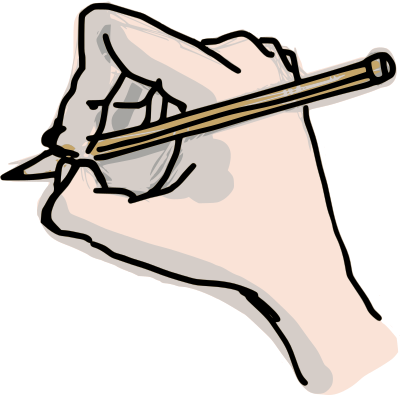
\includegraphics[width=7cm]{imgs/drawingHand.png}};
  \end{tikzpicture}
\end{center}

\noindent\rule{\textwidth}{2pt}

\begin{center}
  Surround to capture.

  \vspace{2cm}
  
  \cleargoban  
  \white{f5}
  \black{f4,g5,e5,f6}
  \largegoban
  \gobansize{9}
  \showgoban[a1,i9]
\end{center}

\newpage

\problem{Black to play. Capture.}{d4}{e4,c4,d5}{How many stones did you capture? \rectangle}{0}{imgs/penguin1.png}{You can do it!}

\noindent\rule{\textwidth}{2pt}

\problem{White to play. Capture.}{f2,g3,e3}{f3}{How many stones did you capture? \rectangle}{1}{imgs/penguin2.png}{Nice work!}

\problem{Black to play. Capture.}{c7}{c6,b7,c8}{How many stones did you capture? \rectangle}{0}{imgs/penguin3.png}{Nice!}

\noindent\rule{\textwidth}{2pt}

\problem{White to play. Capture.}{h9,j8,h7}{h8}{How many stones did you capture? \rectangle}{1}{imgs/penguin4.png}{Get it!}

\problem{Black to play. Capture.}{e9}{d9,e8}{How many stones did you capture? \rectangle}{0}{imgs/penguin5.png}{Watch out!}

\noindent\rule{\textwidth}{2pt}

\problem{White to play. Capture.}{h2,j1}{h1}{How many stones did you capture? \rectangle}{1}{imgs/penguin6.png}{Only 1 stone!}

\problem{Black to play. Capture.}{j5}{h5,j4}{How many stones did you capture? \rectangle}{0}{imgs/penguin7.png}{You can do it!}

\noindent\rule{\textwidth}{2pt}

\problem{White to play. Capture.}{b4,a5}{a4}{How many stones did you capture? \rectangle}{1}{imgs/penguin8.png}{Get it! Get it!}

\problem{Black to play. Capture.}{a1}{a2}{How many stones did you capture? \rectangle}{0}{imgs/penguin9.png}{Only 1 stone!}

\noindent\rule{\textwidth}{2pt}

\problem{White to play. Capture.}{h9}{j9}{How many stones did you capture? \rectangle}{1}{imgs/penguin10.png}{Get it! Get it!}

\problem{Black to play. Capture.}{a9}{b9}{How many stones did you capture? \rectangle}{0}{imgs/penguin11.png}{Only 1 stone!}

\noindent\rule{\textwidth}{2pt}

\problem{White to play. Capture.}{j2}{j1}{How many stones did you capture? \rectangle}{1}{imgs/penguin12.png}{Get it! Get it!}

\problem{Black to play. Defend.}{e4,e6,d5}{e5}{How many stones did you save? \rectangle}{0}{imgs/penguin3.png}{Be careful!}

\noindent\rule{\textwidth}{2pt}

\problem{White to play. Defend.}{f3}{f2,f4,g3}{How many stones did you save? \rectangle}{1}{imgs/penguin3.png}{Save it! Save it!}

\problem{Black to play. Defend.}{a2,b1,c2}{b2}{How many stones did you save? \rectangle}{0}{imgs/penguin3.png}{Quick!}

\noindent\rule{\textwidth}{2pt}

\problem{White to play. Defend.}{h7}{h8,j7,g7}{How many stones did you save? \rectangle}{1}{imgs/penguin3.png}{Save your stone!}

\problem{Black to play. Defend.}{c2,b1}{c1,d2}{How many stones did you save? \rectangle}{0}{imgs/penguin3.png}{Watch out!}

\noindent\rule{\textwidth}{2pt}

\problem{White to play. Defend.}{g9,f8}{g8,h9}{How many stones did you save? \rectangle}{1}{imgs/penguin3.png}{Save your stone!}

\problem{Black to play. Defend.}{b5,a6}{a5,b4}{How many stones did you save? \rectangle}{0}{imgs/penguin3.png}{Watch out!}

\noindent\rule{\textwidth}{2pt}

\problem{White to play. Defend.}{j5,h6}{h5,j4}{How many stones did you save? \rectangle}{1}{imgs/penguin3.png}{Save your stone!}

\problem{Black to play. Defend.}{b9}{a9,b8}{How many stones did you save? \rectangle}{0}{imgs/penguin3.png}{Watch out!}

\noindent\rule{\textwidth}{2pt}

\problem{White to play. Defend.}{j1,h2}{h1}{How many stones did you save? \rectangle}{1}{imgs/penguin3.png}{Save your stone!}

\problem{Black to play. Defend.}{a2}{a1,b2}{How many stones did you save? \rectangle}{0}{imgs/penguin3.png}{Watch out!}

\noindent\rule{\textwidth}{2pt}

\problem{White to play. Defend.}{j9,h8}{j8}{How many stones did you save? \rectangle}{1}{imgs/penguin3.png}{Save your stone!}

\problem{Black to play. Capture.}{d4,d5,d6}{d3,c4,c5,c6,e4,e5,e6}{How many stones did you capture? \rectangle}{0}{imgs/penguin3.png}{Watch out!}

\noindent\rule{\textwidth}{2pt}

\problem{White to play. Capture.}{e2,d3,d4,d5,e6,f6,f3,f4}{e3,e4,e5,f5}{How many stones did you capture? \rectangle}{1}{imgs/penguin3.png}{Get them!}

\problem{Black to play. Capture.}{e1,e2,e3,e4}{d1,d2,d3,d4,f1,f2,f3,f4}{How many stones did you capture? \rectangle}{0}{imgs/penguin3.png}{Watch out!}

\noindent\rule{\textwidth}{2pt}

\problem{White to play. Capture.}{a2,b3,b4,b5,b6,b7,b8}{a3,a4,a5,a6,a7,a8,a9}{How many stones did you capture? \rectangle}{1}{imgs/penguin3.png}{Get them!}


\problem{Black to play. Capture.}{e5,e6}{d5,d6,e4,f4,f6,e7}{How many stones did you capture? \rectangle}{0}{imgs/penguin3.png}{Watch out!}

\noindent\rule{\textwidth}{2pt}

\problem{White to play. Capture.}{d5,d6,e4,f4,f6,e7}{e5,e6,f5}{How many stones did you capture? \rectangle}{1}{imgs/penguin3.png}{Get them!}

\problem{Black to play. Capture.}{f3,f4,g4,g5,h5,h6,j6}{e3,e4,f2,g3,f5,h4,g6,j5,h7}{How many stones did you capture? \rectangle}{0}{imgs/penguin3.png}{Watch out!}

\noindent\rule{\textwidth}{2pt}

\problem{White to play. Capture.}{a7,a8,b9,c8,b6,d7,c5,e6,d4,f5,e3,g4,f2,h3,g1,j2}{b8,b7,c7,c6,d6,d5,e5,e4,f4,f3,g3,g2,h2,h1}{How many stones did you capture? \rectangle}{1}{imgs/penguin3.png}{Get them!}

\problem{Black to play. Capture.}{d3,d4,d5,c3,c5,b3,b4,b5}{a3,a4,a5,e3,e4,e5,b6,c6,d6,b2,c2,d2}{How many stones did you capture? \rectangle}{0}{imgs/penguin3.png}{Watch out!}

\noindent\rule{\textwidth}{2pt}

\problem{White to play. Capture.}{b2,a3,b4,c1,c5,d2,d4,e3}{b3,c4,d3,c2}{How many stones did you capture? \rectangle}{1}{imgs/penguin3.png}{Get them!}

\problem{Black to play. Capture.}{a2,b2,b1}{a3,b3,c2,c1}{How many stones did you capture? \rectangle}{0}{imgs/penguin3.png}{Watch out!}

\noindent\rule{\textwidth}{2pt}

\problem{White to play. Capture.}{b9,b8,c7,d7,e7,f8,f9}{c9,c8,d8,e8,e9}{How many stones did you capture? \rectangle}{1}{imgs/penguin3.png}{Get them!}

\problem{Black to play. Capture.}{c4,b3,c2,d3}{d4,e3,d2}{How many stones did you capture? \rectangle}{0}{imgs/penguin3.png}{Watch out!}

\noindent\rule{\textwidth}{2pt}

\problem{White to play. Capture.}{f6,g7,g5}{h7,j6,h5,g6}{How many stones did you capture? \rectangle}{1}{imgs/penguin3.png}{Get them!}

\problem{Black to play. Capture.}{d9,c8,b9}{e9,d8}{How many stones did you capture? \rectangle}{0}{imgs/penguin3.png}{Watch out!}

\noindent\rule{\textwidth}{2pt}

\problem{White to play. Capture.}{j5,h4}{j4,h3,j2}{How many stones did you capture? \rectangle}{1}{imgs/penguin3.png}{Get them!}

\problem{Black to play. Capture.}{j1,h2,j3}{h1}{How many stones did you capture? \rectangle}{0}{imgs/penguin3.png}{Watch out!}

\noindent\rule{\textwidth}{2pt}

\problem{White to play. Capture.}{b9}{a9,b8,a7}{How many stones did you capture? \rectangle}{1}{imgs/penguin3.png}{Get them!}

\problem{Black to play. Capture.}{c1,d1,e1,f1,g1,d2,e2,f2,e3}{b1,c2,d3,f3,g2,h1}{How many stones did you capture? \rectangle}{0}{imgs/penguin3.png}{Watch out!}

\noindent\rule{\textwidth}{2pt}

\problem{White to play. Capture.}{b1,c2,d3,f3,g2,h1,e4}{c1,d1,e1,f1,g1,d2,f2,e3}{How many stones did you capture? \rectangle}{1}{imgs/penguin3.png}{Get them!}

\problem{Black to play. Defend.}{b1,c2,d3,f3,g2,h1}{c1,d1,e1,f1,g1,d2,e2,f2,e3,e5}{How many stones did you save? \rectangle}{0}{imgs/penguin3.png}{Watch out!}

\noindent\rule{\textwidth}{2pt}

\problem{White to play. Defend.}{c1,d1,e1,f1,g1,d2,f2,e3,c3}{b1,c2,d3,f3,g2,h1,e4,d4}{How many stones did you save? \rectangle}{1}{imgs/penguin3.png}{Get them!}

\problem{Black to play. Capture.}{c3,c7,e5,c5,d4,b6,b7}{g6,g3,e7,d6,d5,c6,b5}{How many stones did you capture? \rectangle}{0}{imgs/penguin3.png}{Watch out!}

\noindent\rule{\textwidth}{2pt}

\problem{White to play. Capture.}{c7,c3,g5,f4,e4,f3,e2}{e5,g3,g7,f6,e3,d4,f2,g2}{How many stones did you capture? \rectangle}{1}{imgs/penguin3.png}{Get them!}

\problem{Black to play. Capture biggest group.}{c3,c4,c5,g1,g2,g3,g4}{b3,b4,b5,c2,c6,d3,d4,f1,f2,f3,f4,h1,h2,h3,h4}{How many stones did you capture? \rectangle}{0}{imgs/penguin3.png}{Watch out!}

\noindent\rule{\textwidth}{2pt}

\problem{White to play. Capture biggest group.}{b1,a2,a3,a4,b5,c5,c1,e2,e3,e4,d1,d5,j1,h2,h3,h4,h5,h6,h7,h8}{b2,b3,b4,c4,c2,d2,d3,d4,j2,j3,j4,j5,j6,j7,j8}{How many stones did you capture? \rectangle}{1}{imgs/penguin3.png}{Get them!}


\end{document}
